\subsubsection{Net 1}
 
\zadatak Re{\sv}i
\begin{align*}
\log_{3x+5}(9x^2+8x+8) &> 2.
\intertext{\resenje Ako se oslobodimo logaritma dobijamo}
9x^2 + 8x + 8 &> (3x + 5)^2\\
9x^2 + 8x + 8 &> 9x^2 + 30x + 25
\intertext{gde je nakon sre{\dj}iva{\nj}a}
\noalign{\vskip-6pt}
x&<-\frac{17}{22}
\intertext{Slede{\cc}i uslov je da osnova bude ve{\cc}a od 1, to jest}
    3x+5 &> 1\\
    x &> -\frac43,
\end{align*}
odakle sledi re{\sv}e{\nj}e
$$
x \in \ram{\left( -\frac43, -\frac{17}{22} \right)}.
$$
% $$
% \slika{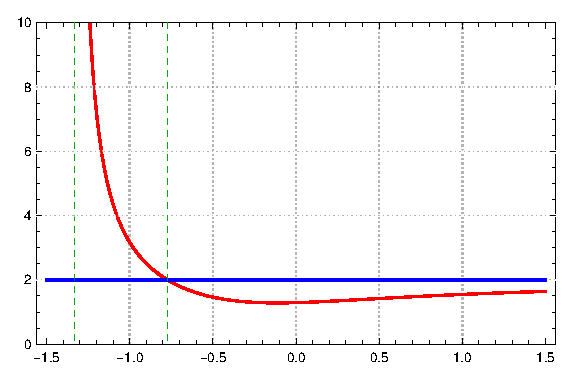
\includegraphics[width=100\mm]{eps/net1.eps}}{$y=\log_{3x+5}(9x^2+8x+8)-2$.}
% $$
